\documentclass[11pt]{beamer}
\usetheme{Berlin}
\usepackage[utf8]{inputenc}
\usepackage[german]{babel}
\usepackage[T1]{fontenc}
\usepackage{amsmath}
\usepackage{amsfonts}
\usepackage{amssymb}
\usepackage{graphicx}
\author{Gruppe C14 \\ Julián Häck, Martin Koytek, Lars Wenning, Erik Zimmermann \\ Vortragender: Lars Wenning}
\setbeamertemplate{footline}[frame number]
%\title{}
%\setbeamercovered{transparent} 
%\setbeamertemplate{navigation symbols}{} 
%\logo{} 
%\institute{} 
%\date{} 
%\subject{} 
\usepackage{subfigure}

\begin{document}

\begin{frame}
\titlepage
\end{frame}

%\begin{frame}
%\tableofcontents
%\end{frame}

\begin{frame}
\section{Gedämpfter LC Schwingkreis, Teilversuch 4.4.2}
\textbf{Gedämpfter LC Schwingkreis Messung mit Cassy, Teilversuch 4.4.2}\centering
\end{frame}

\begin{frame}{Versuchsbeschreibung}
\subsection{Versuchsbeschreibung}
\begin{itemize}
\item Aufzeichnung von mindestens 1 Kriechfall($D=\frac{\delta}{\omega}>1$) und 1 Aperiodischen Grenzfall($D=1$).
\item Messung der Frequenz $f$ und des Dämpfungskoeffizienten $\delta$ nur diesmal mit Sensor-Cassy statt Oszilloskop. Hierzu Messung von Schwingfällen ($D<1$).
\item Bestimmung der frequenz über Fast-Fourier-Transformation(FFT).
\item Bestimmung der Induktivität der Spule aus:
\begin{equation}
\delta =\underbrace{\frac{1}{2L}}_{Steigung}\cdot R
\end{equation}
\end{itemize}
\end{frame}

\begin{frame}{Versuchsaufbau}
\subsection{Versuchsaufbau}
\begin{figure}[H]
    \subfigure[Versuchsaufbau aus dem Skript]{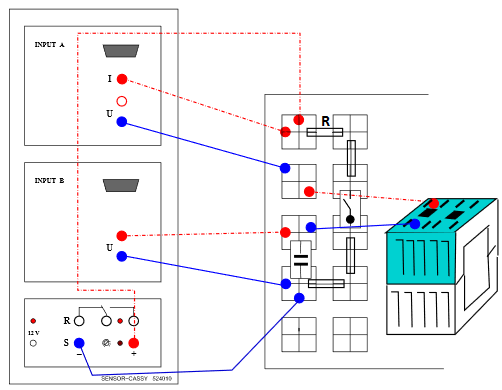
\includegraphics[width=0.49\textwidth]{Bilder/VersuchsaufbauMitWiderstand.PNG}}
    \subfigure[unser Versuchsaufbau mit Widerstand und ohne Strommessung]{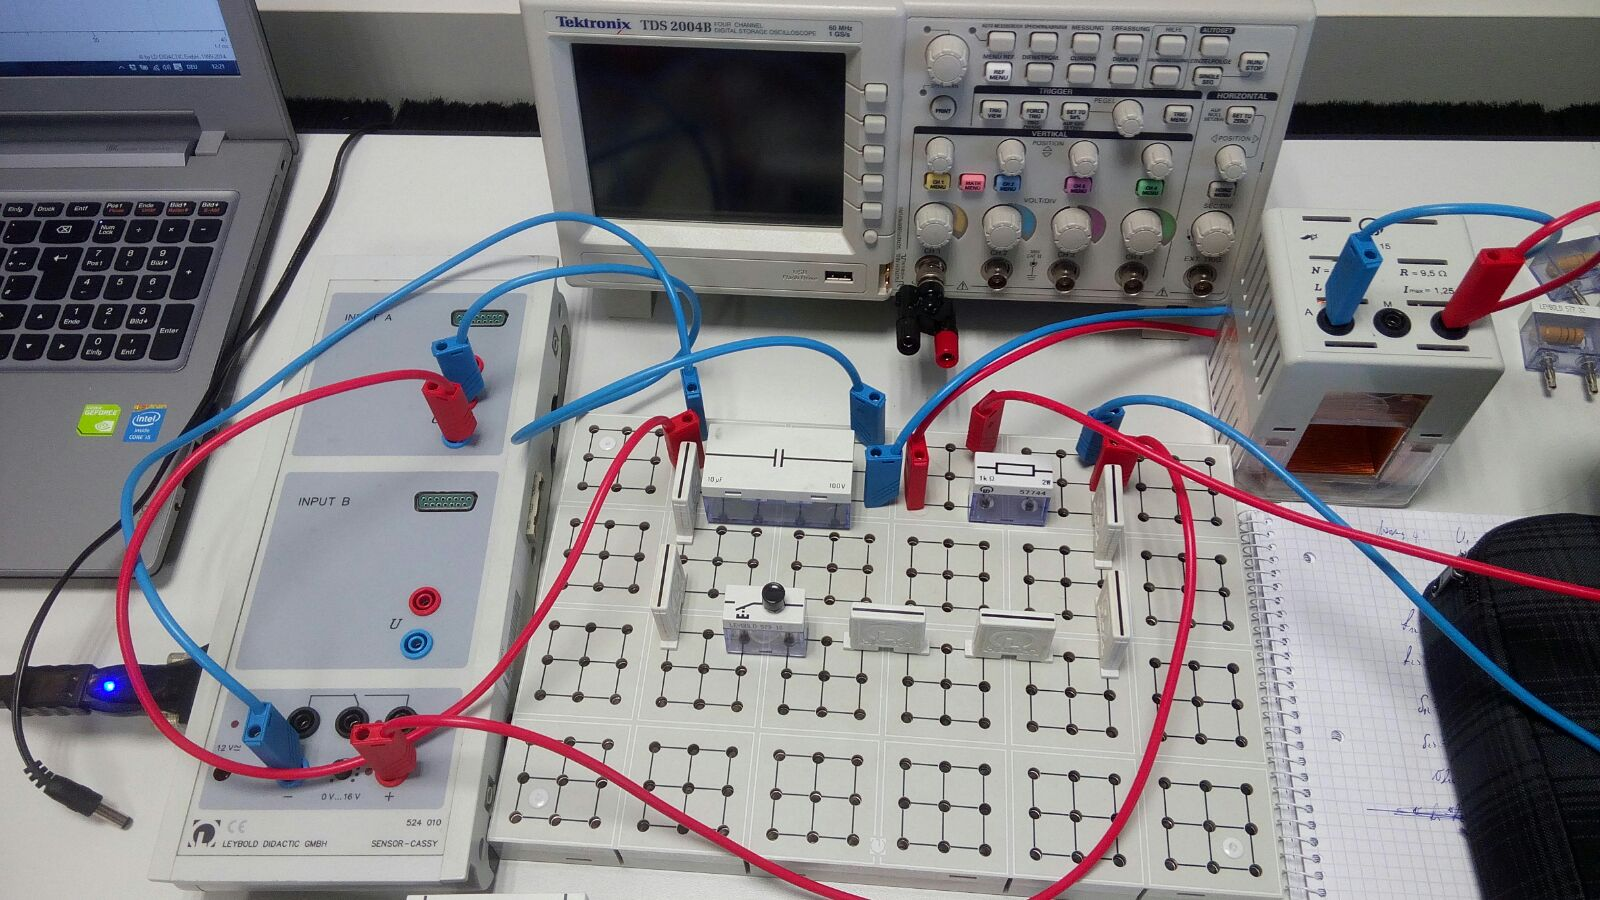
\includegraphics[width=0.49\textwidth]{Bilder/AufbauFoto.jpg}}
\caption{Versuchsaufbau}
\end{figure}
\end{frame}

\begin{frame}{Durchführung}
\begin{itemize}
\subsection{Durchführung}
\item 34 Einzelmessungen.
\item Aufzeichnung des Kriechfalls: Drehwiderstand durch $1k\Omega$ ersetzt.
\item Aufzeichnung des Aperiodischen Grenzfalls: zunächst abgeschätzt:
\begin{equation}
R_{ap}=2\cdot\sqrt{\frac{L}{C}}-R_i\approx 110.5\Omega
\end{equation}
dann Drehwiderstand in diesen Bereich gestellt und gewünschte Charakteristik aufgezeichnet. 
\item für Messung der Frequenz und Dämpfungskoeffizienten Schwingungsmessung über denselben Widerstand. $R\ll R_{ap}$
\item Offsetmessung $\Rightarrow$ verlängerte Messzeit.
\item für Messung der Induktivität unterschiedliche Widerstände über den Drehwiderstand.
\end{itemize}
\end{frame}

\begin{frame}{Auswertung}{Rohdaten}
\subsection{Auswertung}
\subsubsection{Rohdaten}
dieselbe Spule, derselbe Kondensator und dieselbe Eingangsspannung wie in Teilversuch 4.4.1
\begin{figure}[H]
\caption{Schwingfall bei $R\approx 0.02\Omega$ mit Bestimmung des Offsets}
\centering
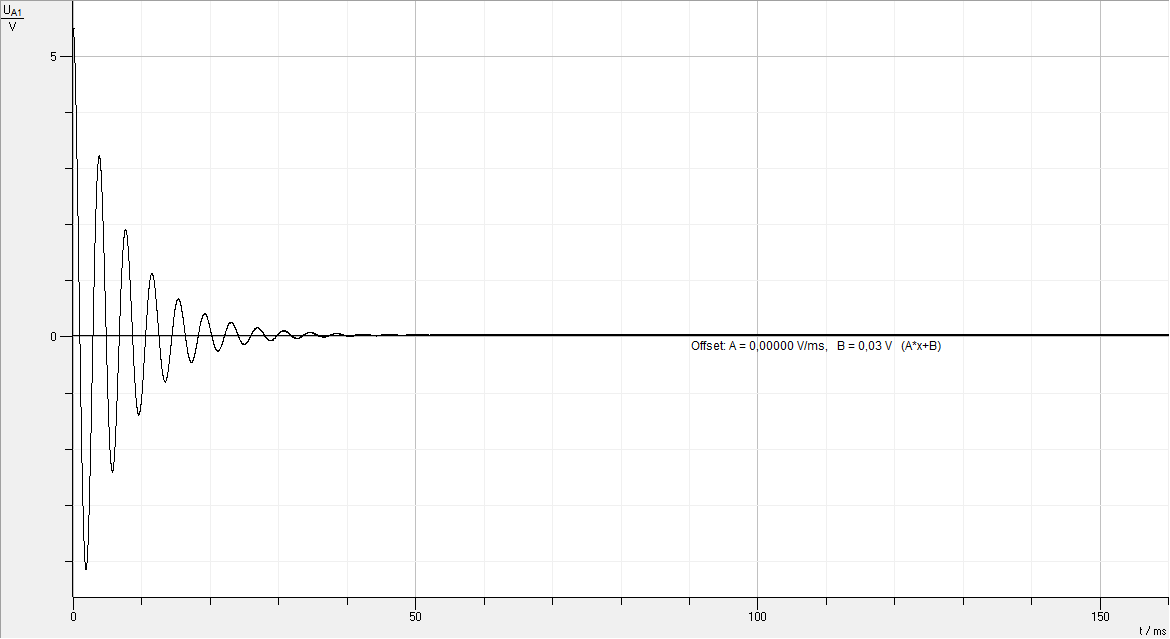
\includegraphics[scale=0.2]{Bilder/SchwingfallMitOffset0Ohm.png}
\end{figure}
\end{frame}

\begin{frame}
\begin{figure}[H]
\caption{Schwingfall bei $2.4\Omega$}
\centering
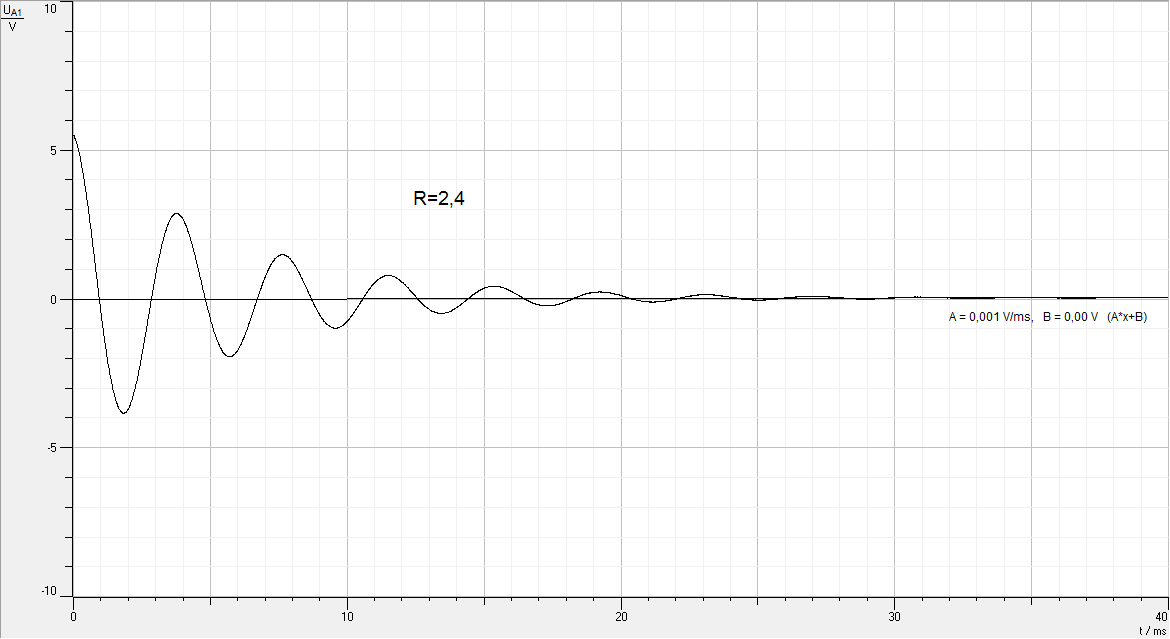
\includegraphics[scale=0.3]{Bilder/Schwingfall2komma4Ohm.png}
\end{figure}
\end{frame}


\begin{frame}
\begin{figure}[H]
\caption{Kriechfall bei R=1k$\Omega$}
\centering
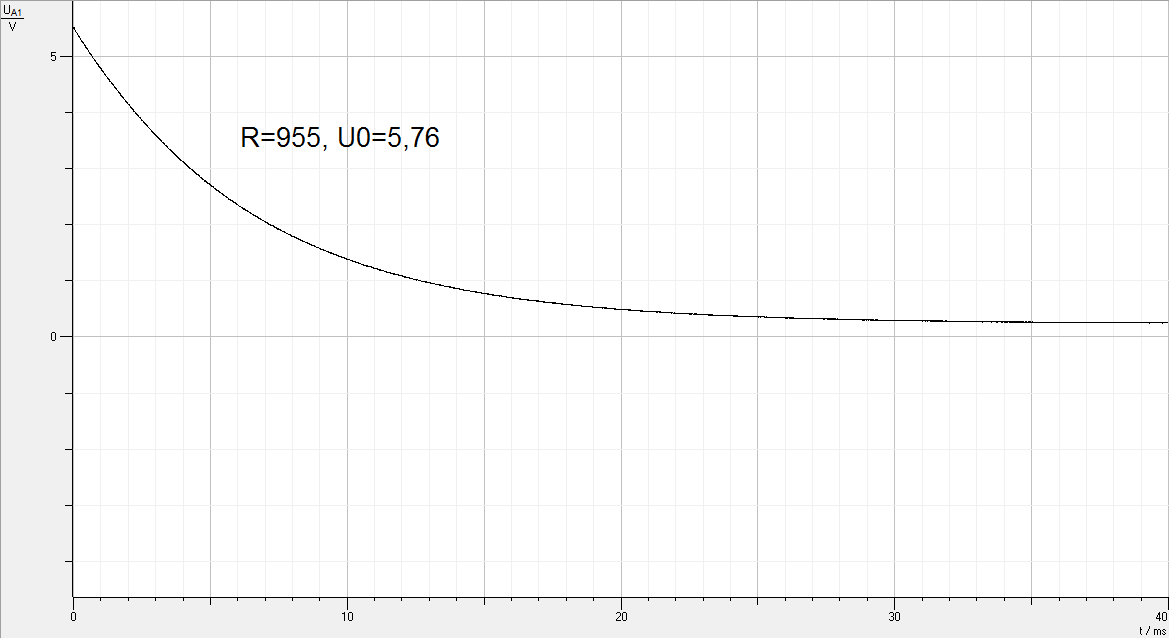
\includegraphics[scale=0.3]{Bilder/Kriechfall1KOhm.png}
\end{figure}
\end{frame}



\begin{frame}{Auswertung}{Transformation der Rohdaten}
\subsubsection{Transformation der Rohdaten}
\begin{figure}[H]
\caption{Bestimmung der Frequenz bei $R=2.4\Omega$ durch FFT}
\centering
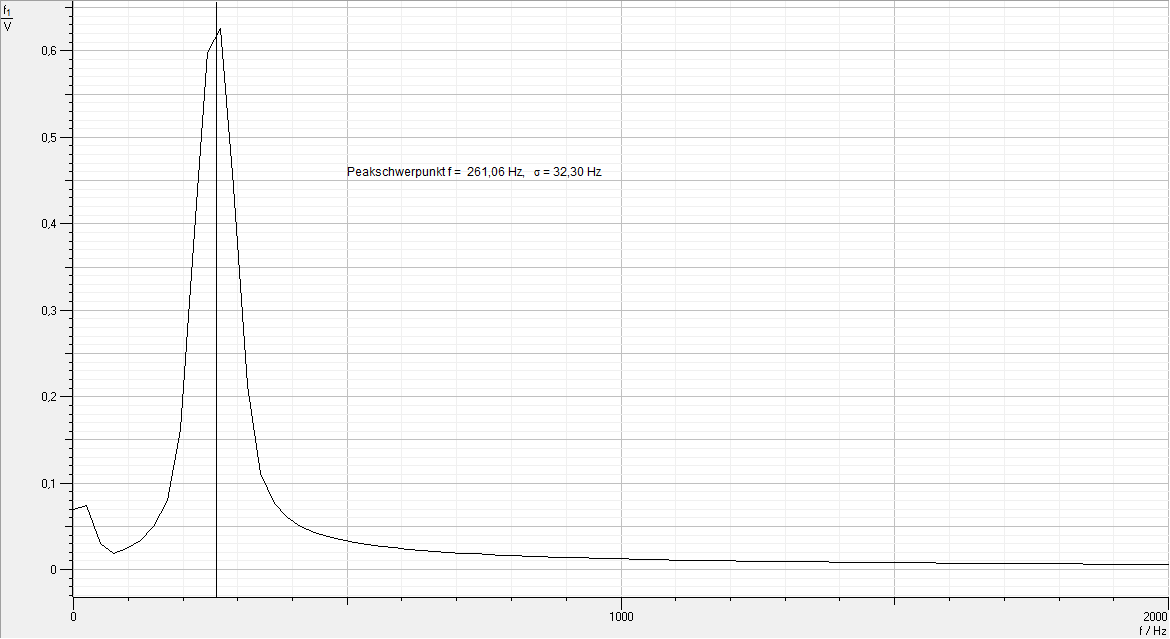
\includegraphics[scale=0.2]{Bilder/PEAK.png}
\end{figure}
\begin{equation}
f=261.06 Hz, \hspace{1cm} \sigma=32,3 Hz.
\end{equation}
\end{frame}

\begin{frame}{Auswertung}{Transformation der Rohdaten}
Bestimmung der Frequenz und des Dämpfungskoeffizienten durch Ablesen.
\begin{figure}[H]
\caption{Messung der Minima und Maxima}
\centering
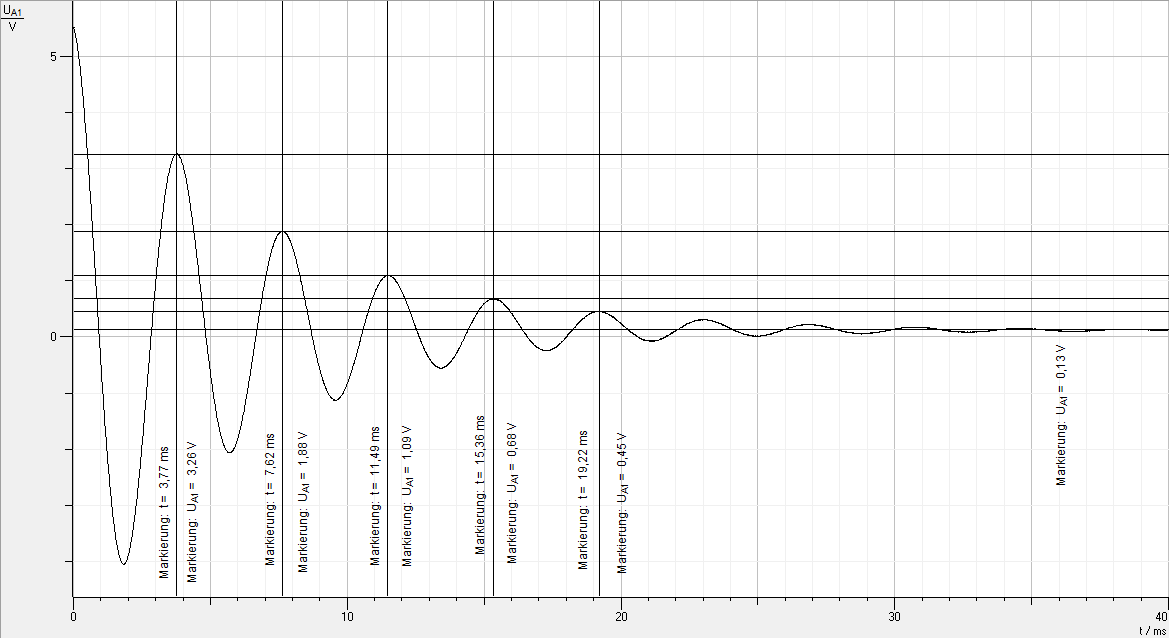
\includegraphics[scale=0.2]{Bilder/Einhuellende.png}
\end{figure}
\end{frame}

\begin{frame}{Auswertung}{Transformation der Rohdaten}
Ergebnisse:
\begin{center}
\begin{tabular}{c|c|c|c|c|c|c}
R in $\Omega$ & $\bar{f}$ in Hz & $\sigma_{\bar{f}}$ in Hz & $f_{Theo}$&  $\bar{\delta}$ in $\frac{1}{s}$ & $\sigma_{\bar{\delta}}$ in $\frac{1}{s}$  & $\delta_{Theo}$ \\ 
\hline 
0.02 & 258.896 & 0.290 & 264.422 & 150.997 & 0.527 & 132.222 \\ 
\hline 
2.4 & 258.398 & 0.334 & 263.951 & 175.023 & 0.654  & 165.278\\ 
\hline 
5.5 & 257.046 & 0.331 & 263.178 & 225.027 & 1.050  & 208.333\\ 
\hline 
11.8 & 254.030 & 0.395 & 261.046 & 285.786 & 1.552  & 295.833 \\ 
\end{tabular} 
\end{center}
\end{frame}

\begin{frame}{Auswertung}{Transformation der Rohdaten}
\begin{figure}[H]
\caption{Bestimmung der Induktivität mittels Linearer Regression}
\centering
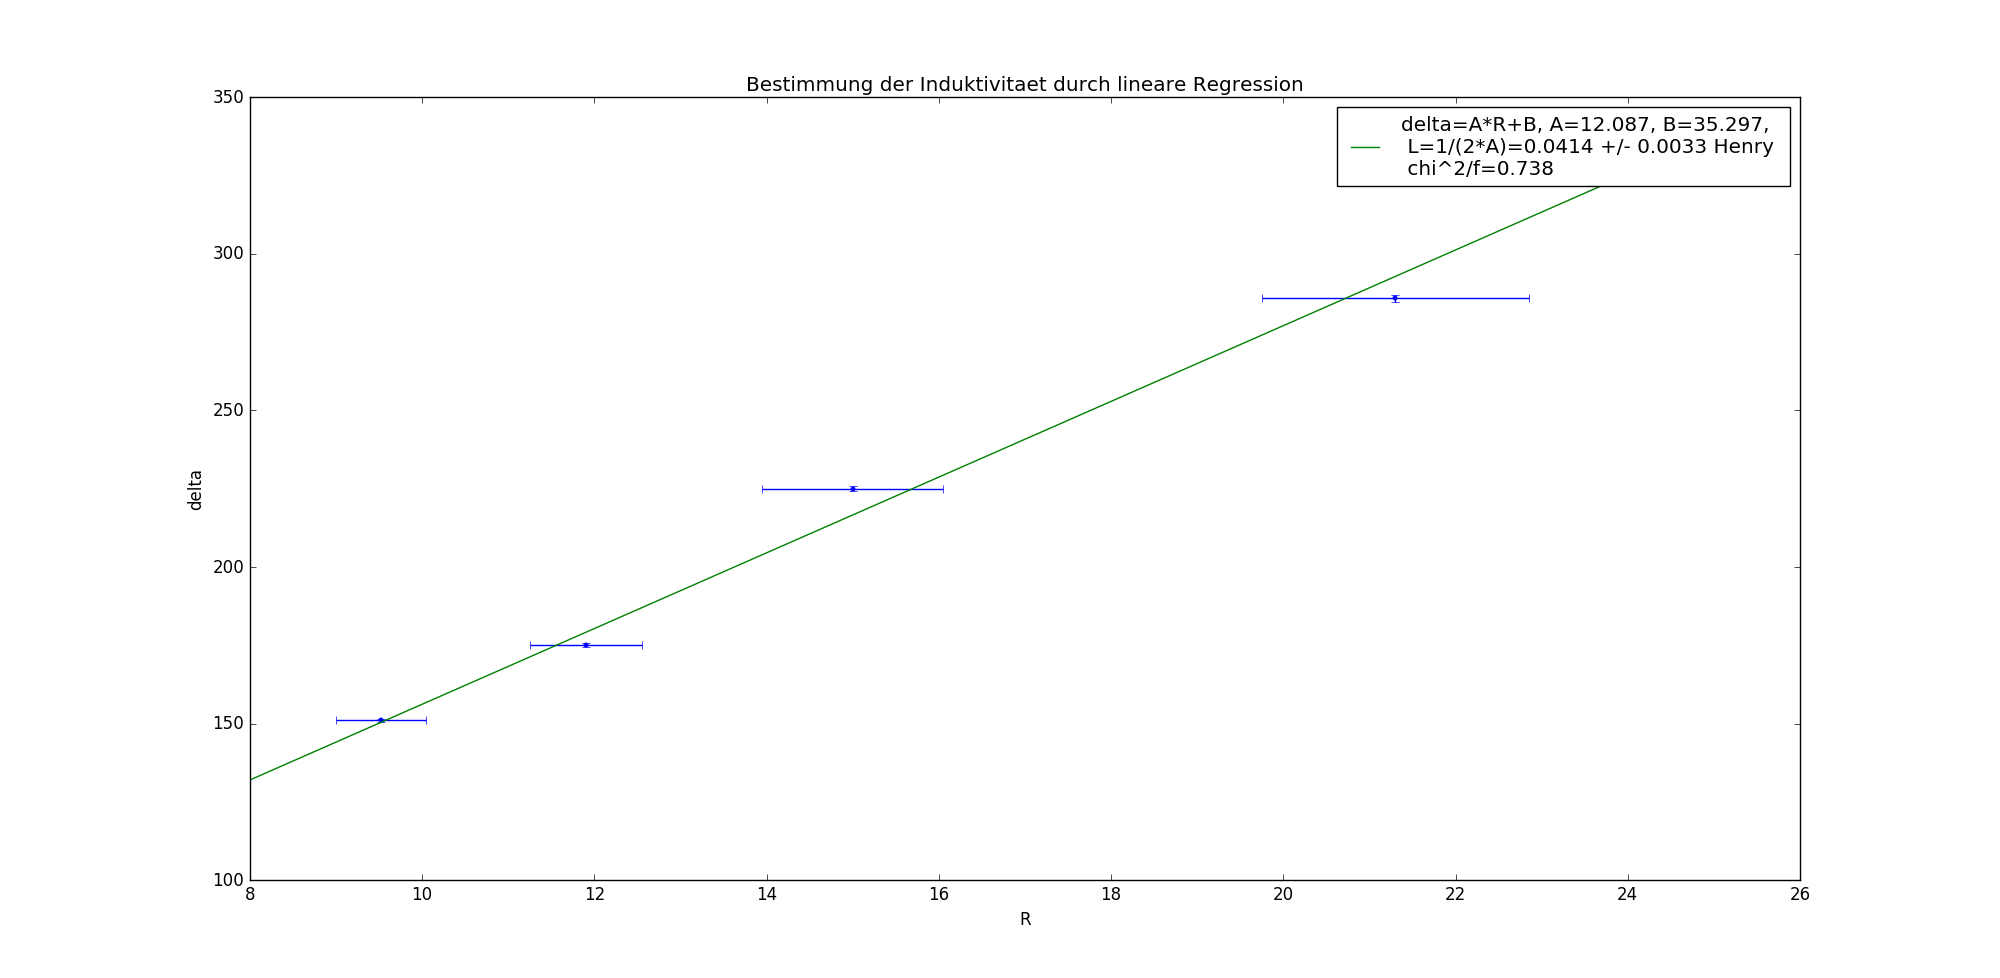
\includegraphics[scale=0.2]{Bilder/Induktivität_linreg.png}
\end{figure}
\end{frame}

\begin{frame}
\begin{figure}[H]
 \caption{Residuenplot für Induktivität}
 \centering
 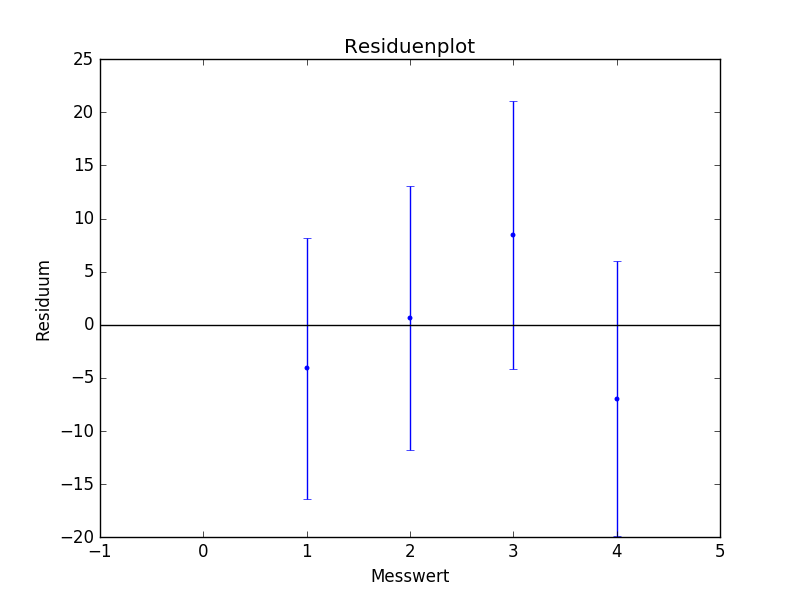
\includegraphics[scale=0.3]{Bilder/ResiduenplotInduktivitaeten.png}
\end{figure}
\end{frame}

\begin{frame}{Auswertung}{Transformation der Rohdaten}
Bestimmung der Induktivität mittels Linearer Regression: \\
Ergebnisse:
\begin{align*}
\delta(R) &= A*R+B \\
A&=12.087 \frac{1}{H} \hspace{1cm} B=35.297 \frac{1}{s} \\
\frac{\chi^2}{f}&=0.738 \\
\Rightarrow L&=\frac{1}{2A}=0.0414 \pm 0.0033 H, \hspace{1cm} L_{Hersteller}=0.036 H
\end{align*}
\end{frame}

\begin{frame}{Auswertung}{Transformation der Rohdaten}
\begin{figure}[H]
\caption{Aperiodischer Grenzfall}
\centering
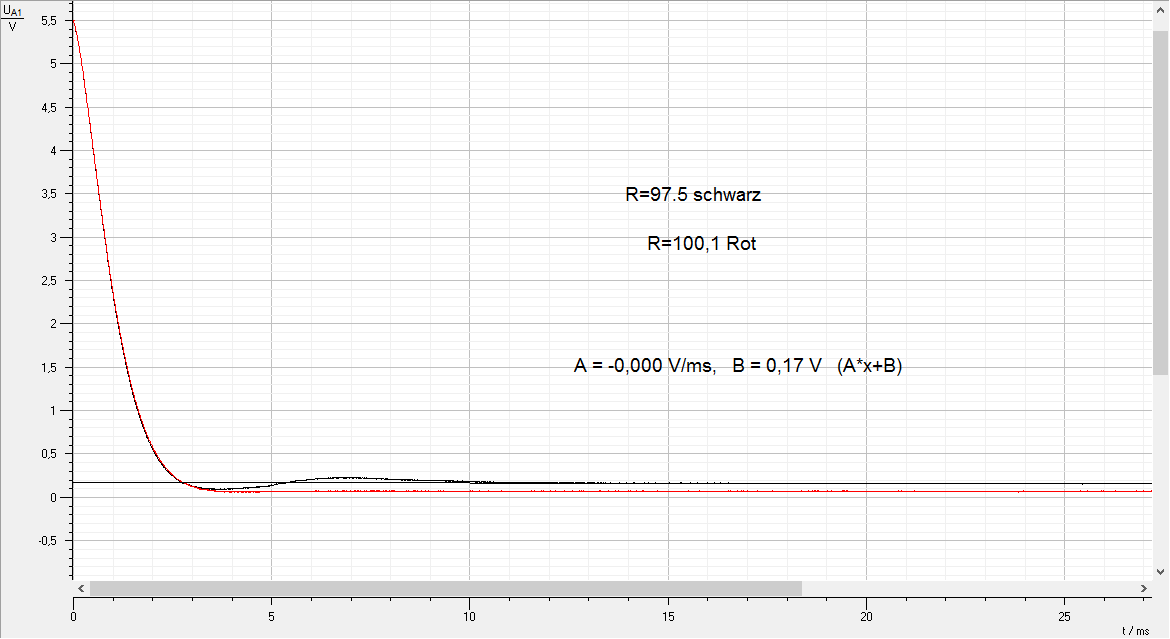
\includegraphics[scale=0.2]{Bilder/AperiodischerGrenzfall.png}
\label{Aperiodisch_Bild}
\end{figure}
\begin{equation}
R_{ap}=100.1\Omega < R_{Theo}\approx 110.5\Omega.
\end{equation}
\end{frame}



\begin{frame}
\textbf{Vielen Dank für ihre Aufmerksamkeit}\centering
\end{frame}
\end{document}